% Estilo general del documento:
	% Tamaño general:
	
	\documentclass[10pt]{beamer}
\setbeamertemplate{footline}[page number]
	\mode<presentation>{
		\usetheme{Hannover}				% Tema de la presentación.
		\usecolortheme[rgb={0.4, 0.2, 1.0}]{structure} 	% Color principal.
		\setbeamercovered{transparent} 			% Con este comando los ítems ocultos se muestran semitransparentes.
		\useinnertheme{rounded}


	}


	% Mostrar el índice de nuevo al cambiar de sección:
	
	\AtBeginSection{
		\begin{frame}<beamer>{\'{I}ndice}
			\tableofcontents[currentsection,subsections]
		\end{frame}
	}
	% Mostrar el índice de nuevo al cambiar de sección:
	
	\AtBeginSubsection{
		\begin{frame}<beamer>{\'{I}ndice}
			\tableofcontents[currentsection, currentsubsection]
		\end{frame}
	}
% Paquetes incluidos por defecto:
	% Tipo de fuente:
	
	\usepackage{palatino}
\usepackage{listings}
\lstset {language=Html, frame=lines, showstringspaces=false}
	% Justificación del texto:
	
	\renewcommand{\raggedright}{\leftskip=0pt \rightskip=0pt plus 0cm} 
	
	% Inclusión de imágenes:
	
	\usepackage{graphicx}
	
	% Matemáticos:

	\usepackage{amsmath, amssymb, latexsym}
	
	% De idioma:
	
	\usepackage[english,spanish]{babel}
	\usepackage[utf8x]{inputenc}
	\usepackage[T1]{fontenc}
	

\title{Videogame analysis}
\author{Jacinto Arias, Adrián Sánchez}
\institute{AI in Videogames \and University of Castilla-La Mancha}
\date{\today}

\begin{document}
\setbeamercolor{background canvas}{bg=black}


\begin{frame}
		\begin{center}
		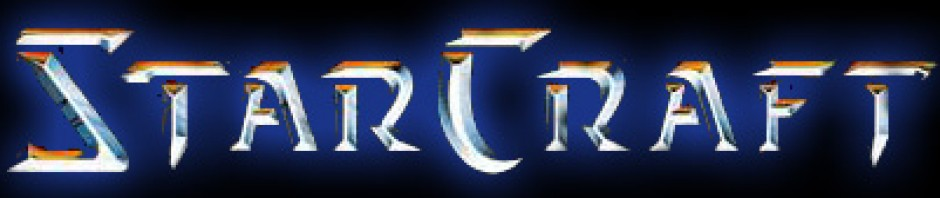
\includegraphics[scale=0.3]{logo.jpg} 
		\end{center}
		\titlepage
\end{frame}


\setbeamercolor{background canvas}{bg=white}


	\begin{frame}{Índice}
		\tableofcontents
	\end{frame}

\section{Origins and repercussion}


\begin{frame}{Origins}
	  \begin{itemize}
	   \item Released on 1998 by Blizzard Entertainment.
	   \item Real Time Strategy.
	   \item Standard for this kind of games.
	   \item More than 11 millions of copies have been sold.

	  \end{itemize}

\begin{center}
	  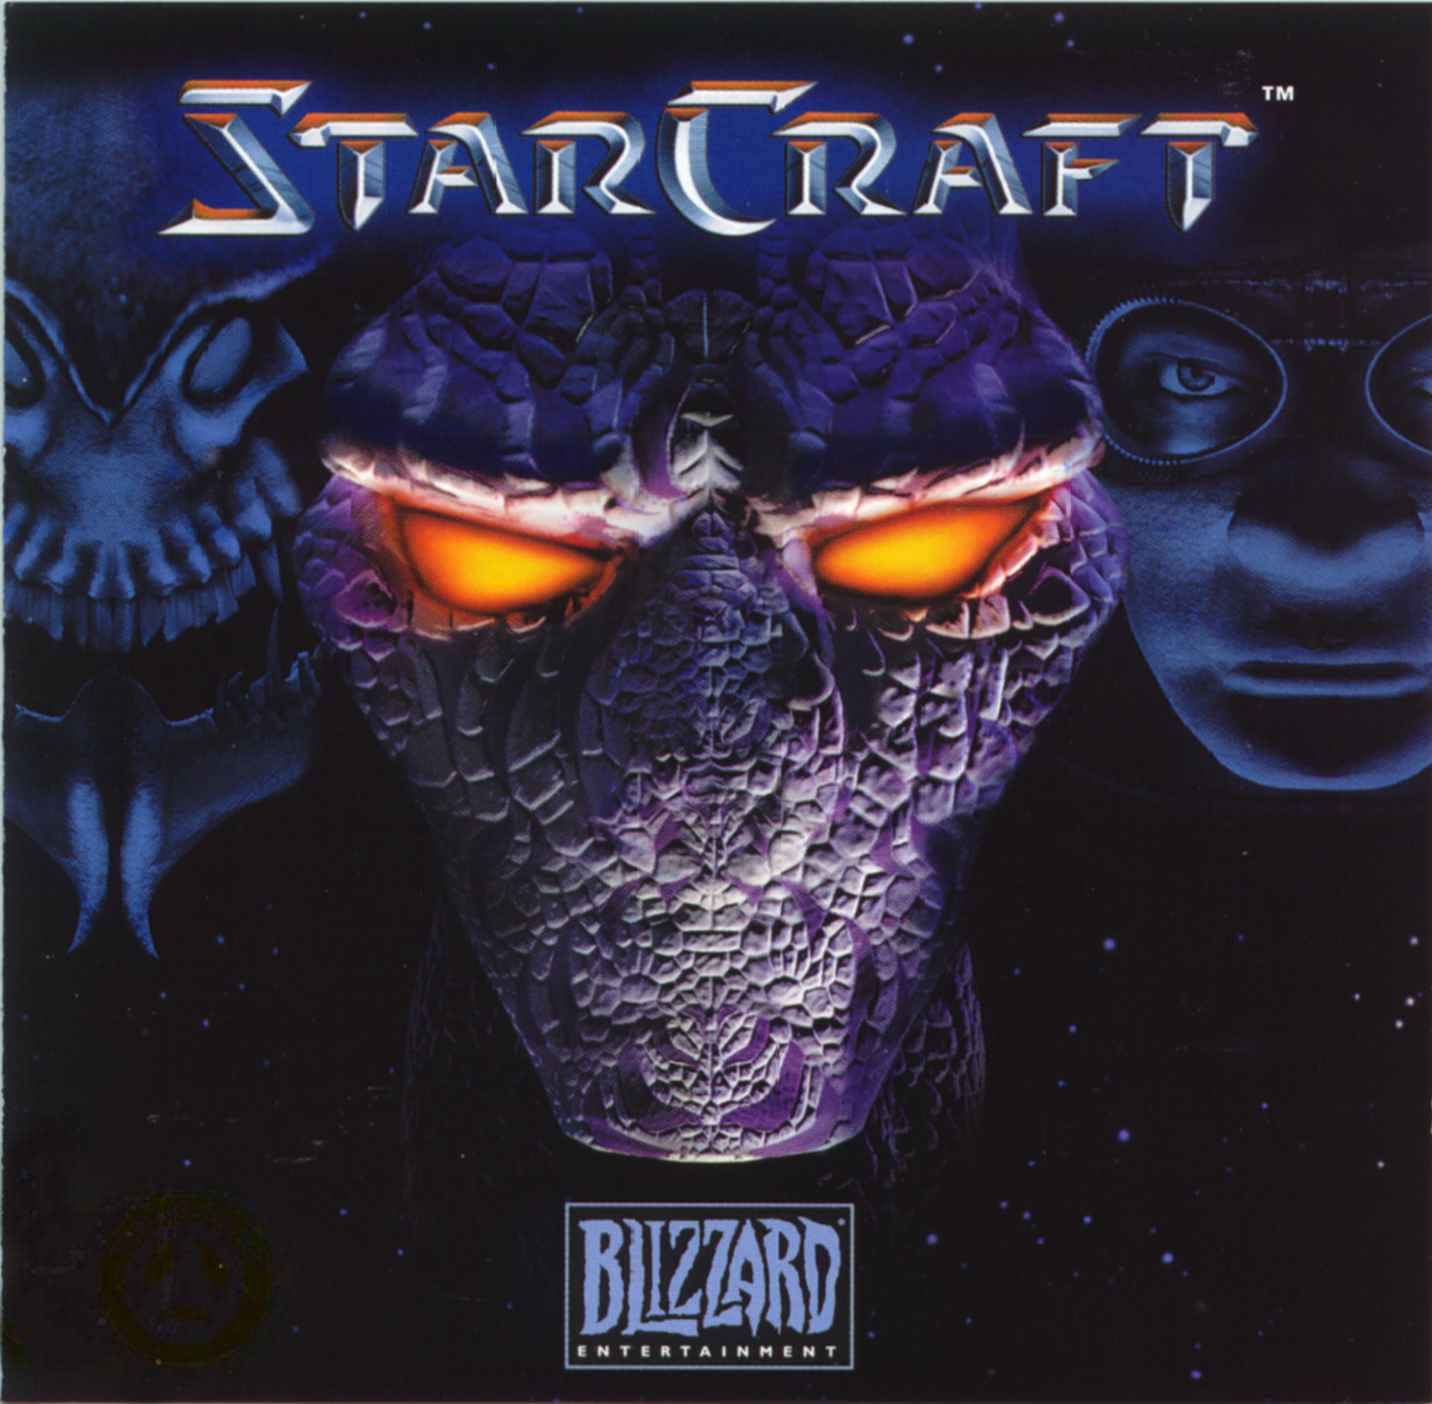
\includegraphics[scale=0.4]{logo1.jpg}\end{center}

\end{frame}

\begin{frame}{Origins}

	  \begin{itemize}
	   \item Works in PC platform both Windows and Mac OS.
	   \item Nintendo64 version was published, didn't became so popular.
	   \item An expansion was published in the same year adding a new campaign and new units (BroodWar).
	   \item In 2010, the expected sequel \textit{Starcraft II: Wings of liberty}, came selling more than 1.5 million copies in the first 48 hours.
	  \end{itemize}
\end{frame}

\begin{frame}{Repercussions}

	  \begin{itemize}
	   \item Starcraft multiplayer has been one the most played games in the internet.
	   \item Blizzard's released its pioneer multiplayer platform \textit{Battle.net}.
	   \item Starcraft can be considered one of the few games that people had been still playing more than 10 years after the release.
	   \item The game's popularity has led to professional players and leagues with sponsorship and televised matches.
	  \end{itemize}
\end{frame}

\section{Features and gameplay}

\begin{frame}{The world of Starcraft}

Starcraft is based on a science-fiction world, where three races fight to take control of a solar system far away from the Earth. The three races are:

    \begin{itemize}
     \item \textbf{Terran:} A technological advanced human society that long time ago moved from earth and get lost in space founding a new independent colony.
     \item \textbf{Protoss:} An elder alien race with advanced society and technology that has became in decadency.
     \item \textbf{Zerg Swarm:} An parasitic insectoid race of aggressive lifeforms that consume planets in order to assimilate the genetic of the native ones.
    \end{itemize}

\end{frame}

\begin{frame}{The world of Starcraft}

\begin{center}
	  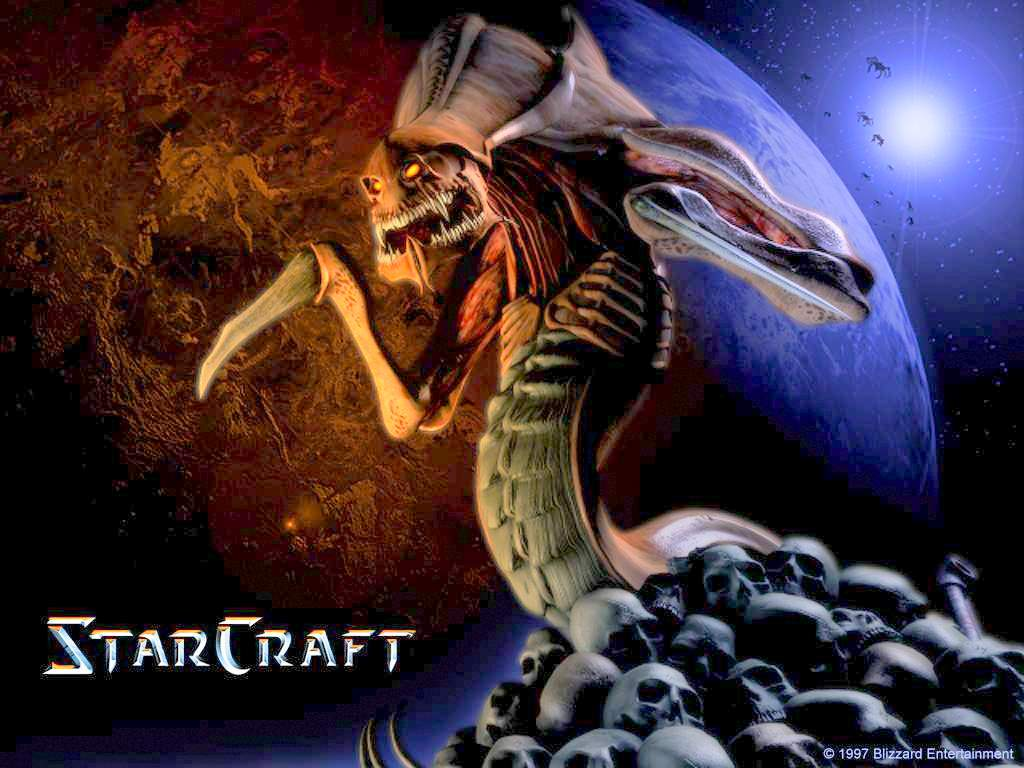
\includegraphics[scale=0.3]{hydralisk.jpg}\end{center}

\end{frame}


\begin{frame}{Game basics}

In order to defeat your opponents you will have to gather resources, build bases and armies and use them against your enemies.

\begin{itemize}
     \item In your screen you will see a portion of the map, you will be able to move along by pushing the screen borders with your mouse.
     \item To control your units and buildings you can select them by pointing with your mouse.
     \item Your units will be able to walk to a different point of the map, to attack other units or patrol some areas.
    \end{itemize}

\end{frame}

\begin{frame}{Game basics}

In Starcraft there are two different kind of games:

    \begin{itemize}
     \item \textbf{Campaign mode}.

    \item \textbf{Multiplayer mode}.
    \end{itemize}

\begin{center}
	  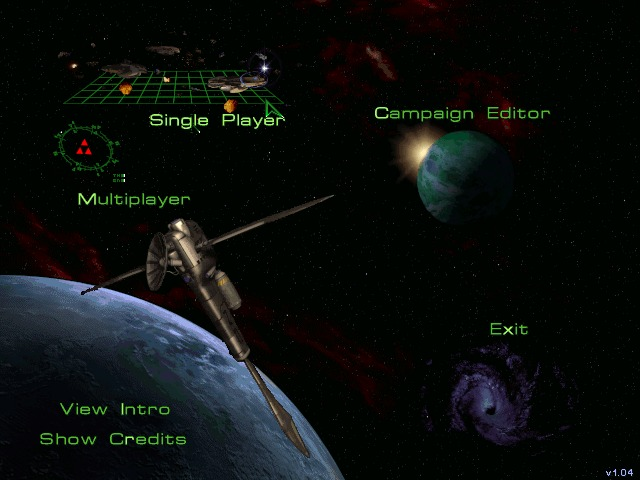
\includegraphics[scale=0.3]{menu.jpg}
\end{center}
\end{frame}

\section{Artificial intelligence principles I: Computational Theory}

\subsection{Game element}
\begin{frame}{Game elements}

In a standard Starcraft game, you will be placed in a map with \textbf{different terrain configurations}.\newline

Also you will find necessary \textbf{resources to gather}.\newline

You will have access to a particular set of \textbf{units} and \textbf{buildings} according to your race, to defeat your opponents.

\begin{center}
	  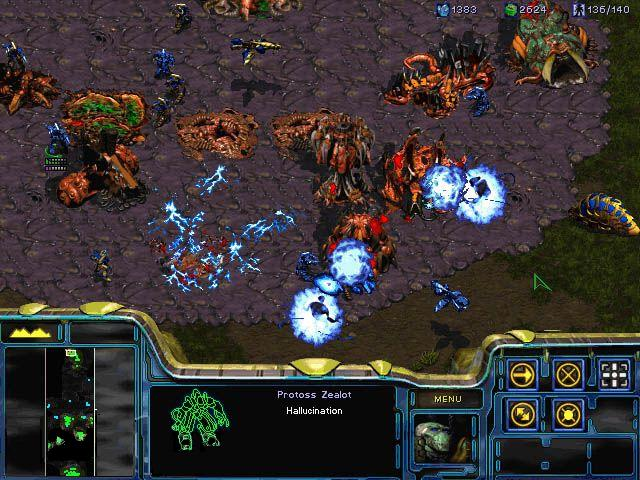
\includegraphics[scale=0.3]{gam1.jpg}
\end{center}
\end{frame}



\begin{frame}{Map, terrain and visibility}

The terrain types condition \textbf{how the units can move around the map}, \small{\textit{i.e a terran marine would walk on the normal ground but it's not allowed to move on the water or lava, however a flying unit will be able to move freely in every type of terrain.}} \newline

Normally, the map is covered in a \textbf{black colour} which represents that you've never visited this area with any unit. Also, there will be areas where the terrain is in a grey colour called \textbf{\textit{war fog}}, so you could not be able to see any of the enemy units in the area, this represents that none of your units can \textit{see} this area.\newline

Each unit has a different \textbf{vision range} which would determine the areas you will see; also, a non flying unit would not be able to see in any terrain higher than the one it is.
\end{frame}


\begin{frame}{Units}

Each race has its set of different units. Every unit in the game has an amount of \textbf{health points}, \textbf{energy}, \textbf{amour} and the majority of them has an \textbf{attack} with its own \textbf{range} and \textbf{damage}. \newline

Each unit is \textbf{stronger} to beat other kinds of units, and is \textbf{weaker} to other kind with no exception, so in order to defeat your enemy you will need to attack him with an optimal army depending of what he has. \newline

Also each race has a \textbf{worker} unit, which is the only unit with can build buildings and gather resources. They are cheap and weak and are the basis of the game economy.
\end{frame}

\begin{frame}{Units}
\begin{center}
	  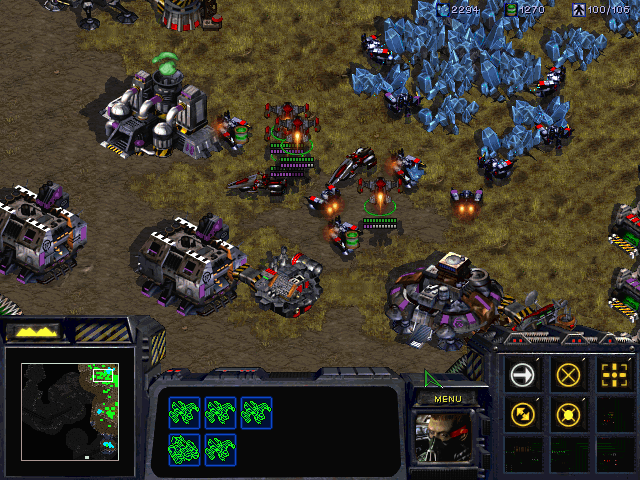
\includegraphics[scale=0.2]{sori.png}
\end{center}
There is two type of units: \textbf{ground} units and \textbf{air} units. The first can only move on the normal terrain and just change to a higher level when using a ramp. \newline

The flying ones could\textbf{ move through every kind of terrain}. \newline

The attack of each unit is defined for ground, air or ground-air targets so it means that some units \textbf{could not be able} to attack specific ones.
\end{frame}


\begin{frame}{Buildings}
A building is like a unit but unlike them are attached to ground and are unmovable and have a great amount of health points. \newline

The buildings purposes include: \textbf{receiving the gathered resources}, \textbf{train units} or do \textbf{researching}. Some structures are \textbf{defensive} so they can attack enemy units.
\end{frame}

\begin{frame}{Resources}
    You will need resources to \textbf{afford} units and buildings.\newline

 Resource is \textbf{gathered} from the map and instantly added to your actual amount. When you build or train units the cost will be \textbf{subtracted} from your amount.\newline

    The game resources are:
    \begin{itemize}
     \item \textbf{Mineral}: most common, gathered from the deposits around the map.
     \item \textbf{Vespene Gas}: less common, it's gathered slowly.
     \item \textbf{Population}: Build special buildings or units to get it. You keep always a maximum level.
    \end{itemize}
\end{frame}

\begin{frame}{Resources}
\begin{center}
	  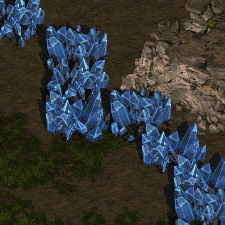
\includegraphics[scale=0.5]{min.jpg}
\end{center}
\begin{center}
	  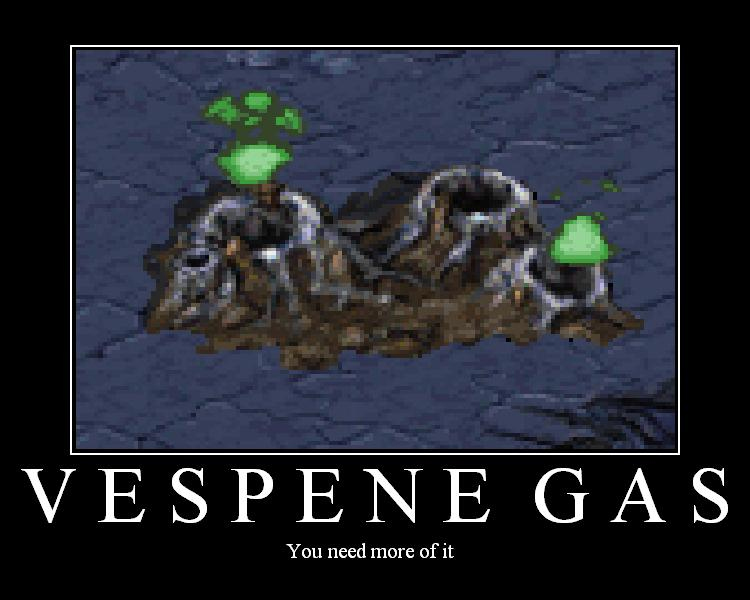
\includegraphics[scale=0.2]{ves.jpg}
\end{center}
\end{frame}

\begin{frame}{Researching and tech tree}
      Each race has an unique \textbf{set of units and buildings}. In order to obtain them the player should meet some \textbf{prerequisites}, commonly it has to build an \textbf{specific building}.\newline

      Some building can do \textbf{researches and upgrades} in order to improve the units or give them a special ability. \newline

Each upgrade costs an amount of resources and takes a lot of time to be completed, but it can \textbf{make a difference} in the game.
\end{frame}

\subsection{Game strategies}


\begin{frame}{Game strategies}
     \begin{itemize}
     \item \textbf{A solid economy is needed}. You will have to explore to find new resources, expand your base and build enough workers to gather resource. A solid economy will allow to have a stronger army.\newline
     \item \textbf{Exploration is fundamental}; when playing this kind of RTS game you should try to know what your opponent is doing at every moment. For this, you will need to continuously explore the map with the fastest units and spy the enemy bases to know which kind of units they have in order to make a proper army to beat them.
\end{itemize}
\end{frame}
\begin{frame}{Game strategies}
\begin{itemize}
     \item \textbf{Build your bases to properly defend them}, \textbf{use buildings and terrain to take advantage}. You can place units behind buildings to defend them and delaying the enemy or place your defences on higher levels to stop the enemy. Also you should take care of the enemy flying units that could infiltrate your bases at any point.\newline
     \item \textbf{Harass your enemy and make all the economic damage you can}. Killing the enemy units is a good point to start but if you don't kill its workers or important buildings he will recover faster and will counter-attack you. Look for defence breaks in order to do as much damage as you can minimizing yours.
    \end{itemize}
\end{frame}

\subsection{Artificial intelligence applications}

\begin{frame}{Artificial intelligence in the game's core}


As Starcraft don't use any advanced physics or 3D perspective to solve, the game core solve this configuring the view in a \textbf{2D isometric perspective} which do trick of making different terrain heights. \newline

The units attack are so simple, since \textbf{no trajectories are calculated} for the ranged shoots, so the impacts are calculated this way: \textit{``If a unit is in range of another, and this one shoots it, the unit get damaged''}.
\end{frame}

\begin{frame}{Artificial intelligence in the game core}
\begin{center}
	  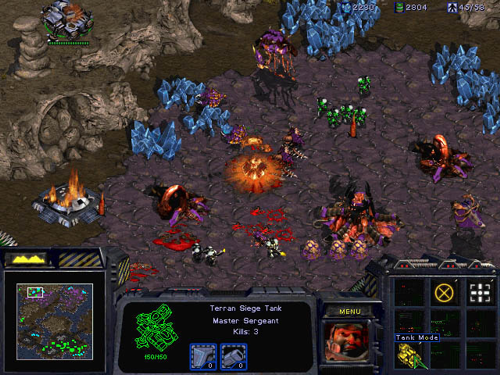
\includegraphics[scale=0.6]{iso.png}
\end{center}
\end{frame}


\begin{frame}{Independent behaviour of each unit}
      \begin{itemize}
       \item When a player order a unit to move somewhere, it has to \textbf{trace a path} and \textbf{follow it across the map} avoiding terrain obstacles, buildings and other units. Also this behaviour gets complicated when more than one unit is doing this.\newline
       \item The units stand in an \textbf{aggressive mode} and have to decide which enemies to shoot when they are in range. Actually in the game, a unit will attack the \textbf{most nearly} enemy unit.
      \end{itemize}
\end{frame}


\begin{frame}{Artificial intelligence as an opponent}
      Whether in campaign or multiplayer mode, \textbf{AI opponents could be added} in order to control one of the players. \newline

      This AI should be able to \textbf{perform all the actions} needed to play in the same way a human would do. \newline

      This include using accordingly all the units of the race chosen, build its base, gather resources, exploring and in summary all the strategies that we told above.
\end{frame}


\begin{frame}{Artificial intelligence as an opponent}
      \textbf{Micro management:} Although the units can act by themselves, the player must order them more precisely if he want to take advantage of their opponents either in combat or moving a big army.\newline

      We are speaking about micro management in the cases of \textbf{ordering your units} to directly attack other specific unit, when \textbf{scouting} the enemy bases or something that requires more \textbf{precise control}.
\end{frame}

\begin{frame}{Artificial intelligence as an opponent}
      \textbf{Macro management:} We speak about macro management when we tell about the player ability to \textbf{produce units}, and keep all of your \textbf{production buildings busy}. Generally, the player with the better macro will have the larger army. \newline

The other element of macro is your ability to \textbf{expand} at the appropriate times to keep your \textbf{production of units flowing}. A good macro player is able to keep increasing his or her production capability while having the \textbf{resources to support it}.
\end{frame}


\section{Artificial intelligence principles II: Representation and algorithms}

\begin{frame}{AIIDE 2010 StarCraft AI Competition}
\begin{center}
	  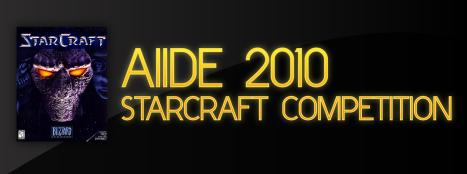
\includegraphics[scale=0.3]{aide.png}
\end{center}
Starcraft was proposed as a \textbf{test platform} to test the latest AI techniques. \newline

In this contest, sponsored by \textbf{Stanford's University} and \textbf{Blizzard Entertainment}, more than \textbf{60 groups} of students of the most important universities competed developing different AI for Stracraft.\newline

The most interesting challenge were the matches \textbf{between AI's}, also, the more advanced played against one of the best human Starcraft players.
\end{frame}

\begin{frame}{AIIDE 2010 StarCraft AI Competition}
\begin{center}
	  \begin{tabular}{cc}
	  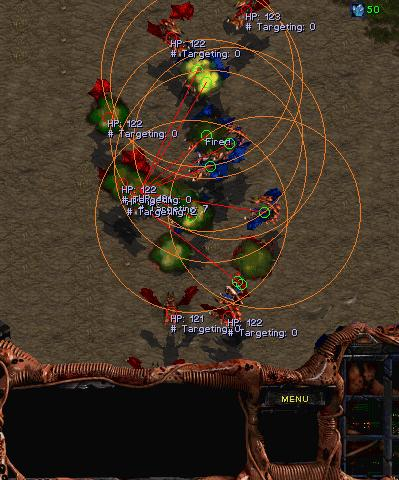
\includegraphics[scale=0.3]{cosa.png} &
	  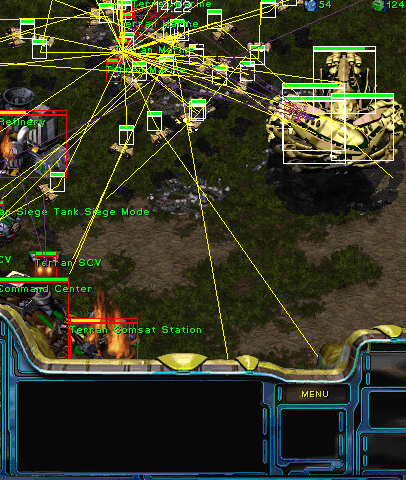
\includegraphics[scale=0.3]{otra.png} 
	  \end{tabular}
	  
\end{center}

\end{frame}

\begin{frame}{AIIDE 2010 StarCraft AI Competition}

  The competition included micro management battles, reduced technology battles and full Starcraft games battles. Some of the technologies used were:

      \begin{itemize}
       \item Finite state machines
       \item Scripting
       \item Dynamic scripting
       \item Probabilistic inference
       \item Influence maps
       \item Neural networks
       \item Swarm intelligence
       \item Potential fields
       \item Genetic programming
      \end{itemize}
\end{frame}

\begin{frame}{AIIDE 2010 StarCraft AI Competition}

Now some videos:

\begin{itemize}
 \item Micro management.
 \item Full battle.
\end{itemize}

\end{frame}



\begin{frame}{The end.}

Thank you for your attention. \newline

	  \begin{center}
	  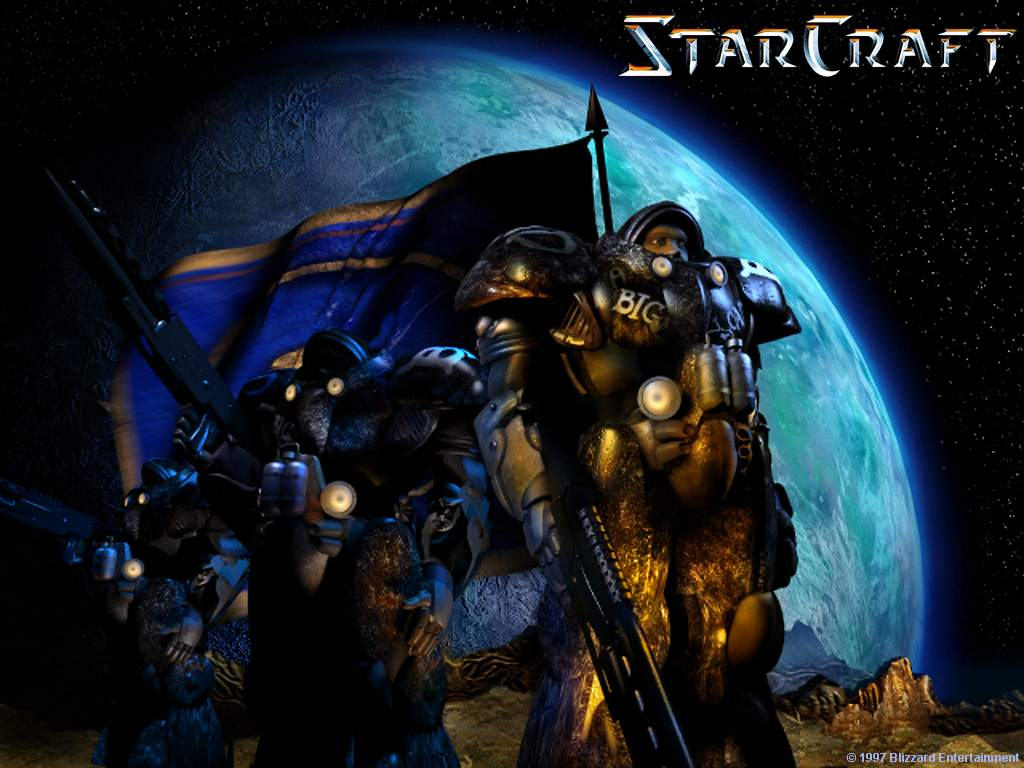
\includegraphics[scale=0.2]{win.jpg}
	  \end{center}


\end{frame}
\end{document}
